\section{Понятие, классификация и принципы работы компьютерных вирусов}
 
\subsection{Определение компьютерного вируса}
 
\textbf{Компьютерный вирус} — это специально написанная, небольшая по размерам программа (т.е. некоторая совокупность выполняемого кода), которая может "приписывать" себя к другим программам ("заражать" их), создавать свои копии и внедрять их в файлы, системные области компьютера и т.д., а также выполнять различные нежелательные действия на компьютере.
 
Программа, внутри которой находится вирус, называется \textbf{заражённой}. Когда такая программа начинает работу, то сначала управление получает вирус. Вирус находит и "заражает" другие программы, а также выполняет какие-нибудь вредные действия (например, портит файлы или таблицу размещения файлов на диске, "засоряет" оперативную память и т.д.). Для маскировки вируса действия по заражению других программ и нанесению вреда могут выполняться не всегда, а, скажем, при выполнении определённых условий.
 
\subsection{Историческая справка}
 
Первые исследования саморазмножающихся искусственных конструкций проводились в середине XX столетия. Термин «компьютерный вирус» появился позднее — официально его автором считается сотрудник Лехайского университета (США) Ф. Коэн в 1984 году на седьмой конференции по безопасности информации.
 
Эксперты считают, что на сегодняшний день число существующих вирусов перевалило за 20 тысяч, причём ежедневно появляется от 6 до 9 новых. «Диких», то есть реально циркулирующих вирусов в настоящее время насчитывается около 260.
 
\begin{figure}[h]
    \centering
    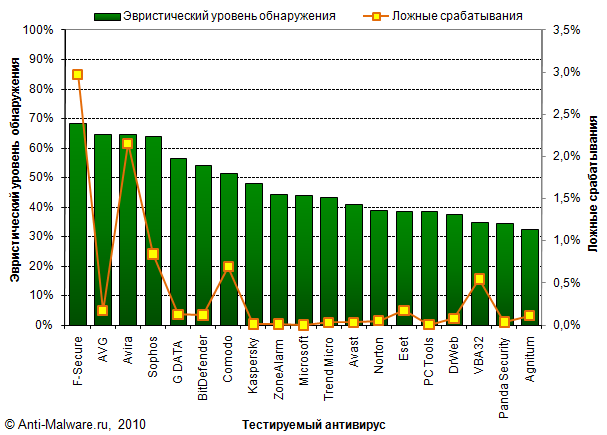
\includegraphics[width=0.7\textwidth]{images/antivirus_comparison.png}
    \caption{Динамика появления новых компьютерных вирусов}
    \label{fig:new_viruses}
\end{figure}
 
\subsection{Классификация компьютерных вирусов}
 
Один из авторитетнейших «вирусологов» страны Евгений Касперский предлагает условно классифицировать вирусы по следующим признакам:
 
\begin{enumerate}
    \item по среде обитания вируса;
    \item по способу заражения среды обитания;
    \item по деструктивным возможностям;
    \item по особенностям алгоритма вируса.
\end{enumerate}
 
\begin{table}[h]
    \centering
    \caption{Классификация компьютерных вирусов по среде обитания}
    \label{tab:classification}
    \begin{tabular}{|c|c|}
        \hline
        \textbf{Тип вируса} & \textbf{Характеристика} \\
        \hline
        Сетевые & Распространяются по компьютерной сети \\
        Файловые & Внедряются в выполняемые файлы \\
        Загрузочные & Внедряются в загрузочный сектор диска (Boot-сектор) \\
        \hline
    \end{tabular}
\end{table}
 
\subsection{Способы заражения}
 
По способу заражения среды обитания вирусы делятся на:
 
\begin{itemize}
    \item \textbf{Резидентные} — находятся в памяти, активны до выключения компьютера;
    \item \textbf{Нерезидентные} — не заражают память, активны ограниченное время.
\end{itemize}
 
\subsection{Деструктивные возможности}
 
По деструктивным возможностям вирусы делятся на:
 
\begin{enumerate}
    \item \textbf{Безвредные} — практически не влияют на работу; уменьшают свободную память на диске в результате своего распространения;
    \item \textbf{Неопасные} — уменьшают свободную память, создают звуковые, графические и прочие эффекты;
    \item \textbf{Опасные} — могут привести к серьёзным сбоям в работе;
    \item \textbf{Очень опасные} — могут привести к потере программ или системных данных.
\end{enumerate}
 
\subsection{Особенности алгоритма вируса}
 
По особенностям алгоритма выделяют следующие типы вирусов:
 
\begin{itemize}
    \item \textbf{Вирусы-«спутники»} — не изменяют файлы, создают для EXE-файлов файлы-спутники с расширением COM;
    \item \textbf{Вирусы-«черви»} — распространяются по сети, рассылают свои копии, вычисляя сетевые адреса;
    \item \textbf{«Паразитические»} — изменяют содержимое дисковых секторов или файлов;
    \item \textbf{«Студенческие»} — примитивны, содержат большое количество ошибок;
    \item \textbf{«Стелс»-вирусы (невидимки)} — перехватывают обращения DOS к поражённым файлам или секторам и подставляют вместо себя незаражённые участки;
    \item \textbf{Вирусы-призраки} — не имеют ни одного постоянного участка кода, труднообнаруживаемы, основное тело вируса зашифровано;
    \item \textbf{Макровирусы} — пишутся не в машинных кодах, а на WordBasic, живут в документах Word.
\end{itemize}
 
\subsection{Как работает вирус: схема функционирования загрузочного вируса}
 
Рассмотрим схему функционирования простого загрузочного вируса, заражающего дискеты. Нормальная схема начальной загрузки выглядит следующим образом:
 
\begin{equation} \label{eq:normal_boot}
    \text{ПНЗ (ПЗУ)} \rightarrow \text{ПНЗ (диск)} \rightarrow \text{СИСТЕМА}
\end{equation}
 
После заражения вирусом в цепочке появляется новое звено:
 
\begin{equation} \label{eq:infected_boot}
    \text{ПНЗ (ПЗУ)} \rightarrow \text{ВИРУС} \rightarrow \text{ПНЗ (диск)} \rightarrow \text{СИСТЕМА}
\end{equation}
 
\begin{figure}[h]
    \centering
    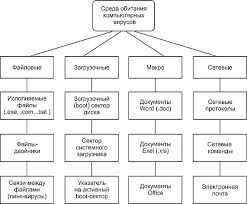
\includegraphics[width=0.6\textwidth]{images/boot_sector.png}
    \caption{Схема заражения загрузочного сектора вирусом}
    \label{fig:boot_sector}
\end{figure}
 
\subsection{Программная реализация: имитация работы вируса}
 
Для демонстрации принципов работы вирусов (в учебных целях) рассмотрим простой скрипт, имитирующий поведение вируса:
 
\begin{listing}[h]
\caption{Имитация поведения вируса на Python}
\label{code:virus_simulation}
 
\begin{minted}[frame=lines,linenos]{python}
class VirusSimulation:
    """Учебная имитация поведения компьютерного вируса"""
    
    def __init__(self, name, destructive_power):
        self.name = name
        self.destructive_power = destructive_power  # от 0 до 10
        self.infected_files = []
        
    def infect(self, filename):
        """Имитация заражения файла"""
        if filename not in self.infected_files:
            self.infected_files.append(filename)
            print(f"Вирус {self.name} заразил файл {filename}")
            return True
        return False
    
    def execute_payload(self, condition):
        """Выполнение вредоносных действий при условии"""
        if condition:
            damage = self.destructive_power * 10
            print(f"Активация вируса! Урон: {damage}%")
            return damage
        return 0
    
    def replicate(self):
        """Имитация размножения"""
        print(f"Вирус {self.name} создал копию себя")
        return VirusSimulation(f"{self.name}_copy", self.destructive_power)
 
# Пример использования
virus = VirusSimulation("TestVirus", 7)
virus.infect("program.exe")
virus.infect("program.exe")  # Повторное заражение не происходит
virus.execute_payload(True)
virus.replicate()
\end{minted}
\end{listing}